% !TeX root = ../Skript_HTML.tex
\cohead{\Large\textbf{Tabellen}}
\section{Tabellen}
Bei der Gestaltung einer Website sollte immer die Übersichtlichkeit im Vordergrund stehen. Um Inhalte, Schrift oder Bilder strukturiert darstellen zu können, benötigt man häufig Tabellen. Mit Hilfe einer Tabelle kann man z.B. den Stundenplan übersichtlich darstellen.

\begin{Exercise}[title=Erstelle deinen Stundenplan in \textit{stundenplan.html}, label=Tabellen1]
    \begin{enumerate}
        \item Informiere dich über Tabellen. Beachte dabei den Unterschied zwischen Tabellenüberschriften und normalen Tabellendaten.
        \item Erstelle einen Beispielstundenplan (Bsp. siehe Bilder weiter unten).
        \item Verbinde alle Zellen der letzten Spalte und füge eine Verlinkung zu \textit{schueler.html} ein.
    \end{enumerate}
\end{Exercise}
Deine Webseite sollte dann ungefähr so aussehen:

\begin{minipage}[t]{\textwidth}
    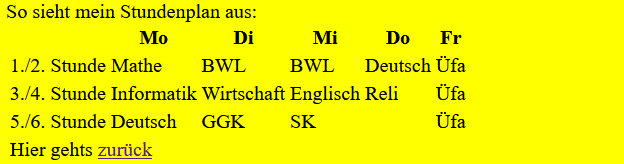
\includegraphics[width=0.8\linewidth]{\pics/TabelleOhneFormatierung.png}
\end{minipage}%

\begin{Exercise}[title=Formatiere deine Tabelle mit Hilfe von CSS, label=Tabellen2]
    \begin{enumerate}
        \item Der Inhalt der Tabelle soll zentriert sein.
        \item Die Tabelle und die einzelnen Zellen sollen schwarze Gitternetzlinien bekommen.
        \item Die Tabellenüberschriften sollen kursiv sein.
        \item Die Tabellenüberschriften und -inhalte sollen blau sein.
        \item Die Tabelle soll zentriert und 800px breit sein.
        \item Validiere dann deine Datei \textit{stundenplan.html}.
    \end{enumerate}
\end{Exercise}

\begin{minipage}[t]{\textwidth}
    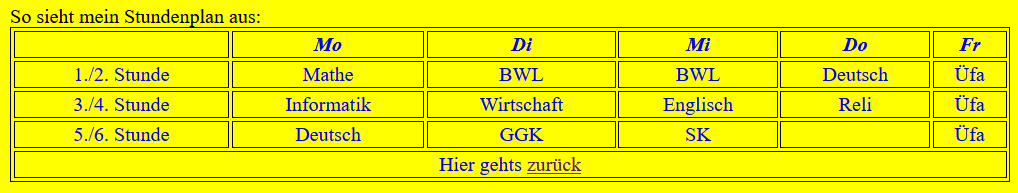
\includegraphics[width=\linewidth]{\pics/TabelleMitFormatierung.png}
\end{minipage}%